%\RequirePackage[2020-02-02]{latexrelease}
\documentclass[a4paper,twoside,12pt]{report}
 %openright
\newcommand{\documenttype}{Report 1}
\newcommand{\thesistitle}{Elektriske Energisystemer i Praksis}
\newcommand{\thesissubtitle}{Metaldetektor}

\newcommand{\thesisauthor}{Gruppe 11} % Your name :) 
\newcommand{\studentnumber}{s111111}
\newcommand{\thedate}{20 Juni 2023} % For example "June, 2019"

\newcommand{\department}{62768}
\newcommand{\departmentdescriber}{Elektriske energisystemer}
\newcommand{\addressI}{Brovej, Building 118}
\newcommand{\addressII}{2800 Kgs. Lyngby}
\newcommand{\departmentwebsite}{www.byg.dtu.dk}
%\usepackage{microtype}      % better looking text
\usepackage[table]{xcolor}
\usepackage{fontspec}       % Package for custom fonts
\usepackage[]{geometry}     % Package for changing page margins (before fancyhdr) 
\usepackage{fancyhdr}       % Package to change header and footer
\usepackage{tocloft}
\usepackage{parskip}        % Package to tweak paragraph skipping (instead of indents a small skip is added after every paragraph)
\usepackage{titlesec}
\usepackage{tikz}           % Package for drawing
\usepackage{pgfplots}       % Package for creating graphs and charts
\usepackage{xcolor}         % Package for defining DTU colours to be used

\usepackage{amsmath}        % For aligning equations among other
\usepackage{siunitx}        % SI units

\usepackage{listings}       % Package for inserting code, (before cleveref)
\PassOptionsToPackage{hyphens}{url} % Ability to line break urls at hyphens
\usepackage{hyperref}       % Package for cross referencing (also loads url package)
\usepackage{cleveref}       % improved cross referencing
\usepackage{textcomp}       % \textdegree = °C and other useful symbols
\usepackage{textgreek}
\usepackage[danish]{babel} % localisation 
\usepackage{caption}        % better captions
\usepackage{subcaption}     % for subfigures
%\usepackage{csquotes}       % For biblatex with babel
%\usepackage[backend=biber,style=authoryear,sorting=none]{biblatex} % Package for bibliography (citing)
\bibliography{bibliography.bib}
\usepackage{tabularx}       % for ability to adjust column spacing in tabular better
\usepackage{booktabs}       % for better tables
%\captionsetup[table]{name=Tabel} % for changing the table navn to fx danish.
%\captionsetup[figure]{name=Figur} % for changing the figur navn to fx danish.
\usepackage{float}          % floating figures in correct places
\usepackage{calc}           % Adds ability for latex to calculate (3pt+2pt) 
\usepackage{blindtext}
%\usepackage{contour}
\usepackage[final]{pdfpages}
\usepackage{minted}
\usepackage{subfiles} % Best loaded last in the preamble
\usepackage[export]{adjustbox}
\usepackage{longtable}
\usepackage{pgf-pie}

\usepackage{wrapfig}

% Colours! 
\newcommand{\targetcolourmodel}{cmyk} % rgb for a digital version, cmyk for a printed version. Only use lowercase
\selectcolormodel{\targetcolourmodel}

% Define colours from https://www.designguide.dtu.dk/
\definecolor{dtured}    {rgb/cmyk}{0.6,0,0 / 0,0.91,0.72,0.23}
%\definecolor{blue}      {rgb/cmyk}{0.1843,0.2431,0.9176 / 0.88,0.76,0,0}
\definecolor{brightgreen}{rgb/cmyk}{0.1216,0.8157,0.5098 / 0.69,0,0.66,0}
\definecolor{navyblue}  {rgb/cmyk}{0.0118,0.0588,0.3098 / 1,0.9,0,0.6}
%\definecolor{yellow}    {rgb/cmyk}{0.9647,0.8157,0.3019 / 0.05,0.17,0.82,0}
\definecolor{orange}    {rgb/cmyk}{0.9882,0.4627,0.2039 / 0,0.65,0.86,0}
\definecolor{pink}      {rgb/cmyk}{0.9686,0.7333,0.6941 / 0,0.35,0.26,0}
\definecolor{grey}      {rgb/cmyk}{0.8549,0.8549,0.8549 / 0,0,0,0.2}
%\definecolor{red}       {rgb/cmyk}{0.9098,0.2471,0.2824 / 0,0.86,0.65,0}
%\definecolor{green}     {rgb/cmyk}{0,0.5333,0.2078 / 0.89,0.05,1,0.17}
\definecolor{purple}    {rgb/cmyk}{0.4745,0.1373,0.5569 / 0.67,0.96,0,0}

\definecolor{light-gray}{gray}{0.95}
\definecolor{med-gray}{gray}{0.85}

\newcommand{\dtulogocolour}{white} % Colour of the DTU logo: white, black or dtured
\newcommand{\frontpagetextcolour}{white} % front page text colour: white or black
\colorlet{frontbackcolor}{navyblue} % Set the background colour of the front- and back page. Choose the colour so it matches the main colour of front page picture

% DTU colours for diagrams
% You might want to make the front/back page background colour the first colour in the plot cycle list.
\pgfplotscreateplotcyclelist{DTU}{%
dtured,         fill=dtured,        \\%
blue,           fill=blue,          \\%
brightgreen,    fill=brightgreen    \\%
navyblue,       fill=navyblue       \\%
yellow,         fill=yellow         \\%
orange,         fill=orange         \\%
grey,           fill=grey           \\%
red,            fill=red            \\%
green,          fill=green          \\%
purple,         fill=purple         \\%
}


% Font
% There is no corporate serif font in the DTU design guide. The DTU design team has proposed to use Neo Sans for headings - and Arial for the body text.
% To change heading font to NeoSans Pro please upload both NeoSansPro-Regular.otf and NeoSansPro-Medium.otf to the root directory.
\setmainfont{Arial}
\renewcommand\thepart{Part \Roman{part}}
\IfFontExistsTF{NeoSansPro-Medium.otf}
{ %If True set headings to NeoSans Pro
\newfontface\NeoSansProReg{NeoSansPro-Regular.otf}
\newfontface\NeoSansProMed{NeoSansPro-Medium.otf}
\titleformat{\part}[display]{\NeoSansProMed \huge \centering}{\NeoSansProMed \Huge \thepart}{1em}{\thispagestyle{empty}}{}
\titleformat{\chapter}{\NeoSansProMed\huge}{\thechapter}{1em}{\raggedright}
\titleformat{\section}{\NeoSansProMed\Large}{\thesection}{1em}{\raggedright}
\titleformat{\subsection}{\NeoSansProMed\large}{\thesubsection}{1em}{\raggedright}
\titleformat{\subsubsection}{\NeoSansProMed\normalsize}{\thesubsubsection}{1em}{\raggedright}
\newcommand\TitleFont[1]{{\NeoSansProMed #1}}
\newcommand\titlefont[1]{{\NeoSansProReg #1}}
}
{ % If false
\titleformat{\part}[display]{\bfseries\huge \centering}{\bfseries\Huge \thepart}{1em}{\thispagestyle{empty}}{}
\titleformat{\chapter}{\bfseries\huge}{\thechapter}{1em}{\raggedright}
\titleformat{\section}{\bfseries\Large}{\thesection}{1em}{\raggedright}
\titleformat{\subsection}{\bfseries\large}{\thesubsection}{1em}{\raggedright}
\titleformat{\subsubsection}{\bfseries\normalsize}{\thesubsubsection}{1em}{\raggedright}
\newcommand\TitleFont[1]{{\bfseries #1}}
\newcommand\titlefont[1]{{#1}}
}
\urlstyle{sf}
%\def\UrlFont{\NeoSansProReg}


% If you wish to use the pdflatex compiler, sans-serif Helvetica can be used as a replacement for Arial. In this way you will be able to use the microtype package. Remember to add \usepackage[utf8]{inputenc} and disable the fontspec package. 
%\newcommand\TitleFont[1]{{\bfseries #1}}
%\newcommand\titlefont[1]{{#1}}
%\fontfamily{qhv}\selectfont
%\renewcommand{\familydefault}{\sfdefault}


% Watermark for confidential or draft (or anything else)
%\sffamily % set the correct font for the watermark
\newsavebox\mybox
\savebox\mybox{\tikz[color=grey,opacity=0.5]\node{Template};}

% Table of contents (TOC) and numbering of headings


\renewcommand{\cftchapleader}{\cftdotfill{\cftdotsep}} % for chapters
\setlength{\cftsecindent}{3mm}
\setlength{\cftsubsecindent}{7mm}
\setcounter{tocdepth}{1}    % Depth of table of content: sub sections will not be included in table of contents (1=chapter, 2 = section etc.)
\setcounter{secnumdepth}{2} % Depth of section numbering: sub sub sections are not numbered

\makeatletter % Reset chapter numbering for each part
\@addtoreset{chapter}{part}
\makeatother  

% Spacing of titles and captions
\titlespacing\chapter{0pt}{0pt plus 0pt minus 0pt}{0pt plus 0pt minus 0pt}
\titlespacing\section{0pt}{12pt plus 0 pt minus 0 pt}{0pt plus 0pt minus 0pt}
\titlespacing\subsection{0pt}{8pt plus 0pt minus 0pt}{0pt plus 0pt minus 0pt}
\titlespacing\subsubsection{0pt}{4pt plus 0pt minus 0pt}{0pt plus 0pt minus 0pt}
\captionsetup{belowskip=\parskip,aboveskip=0pt plus 0pt minus 0pt}

% Setup header and footer
\fancypagestyle{main}{% All normal pages
    \fancyhead{}
    \fancyfoot{}
    \renewcommand{\headrulewidth}{0pt}
    \fancyfoot[LE,RO]{\footnotesize \thepage}
    \fancyfoot[RE,LO]{\footnotesize \thesistitle} % - \rightmark
    \fancyhfoffset[E,O]{0pt}
}
\fancypagestyle{plain}{% Chapter pages
    \fancyhead{}
    \fancyfoot{}
    \renewcommand{\headrulewidth}{0pt}
    \fancyfoot[LE,RO]{\footnotesize \thepage}
    \fancyfoot[RE,LO]{\footnotesize \thesistitle} % - \leftmark
    \fancyhfoffset[E,O]{0pt}
}

% Setup for diagrams and graphs (tikz pictures) 
\usetikzlibrary{spy}    % For magnifying anything within a tikzpicture, see the line graph
\usepgfplotslibrary{statistics} % Package for the boxplot
\pgfplotsset{ % Setup for diagrams
compat=newest,
major x grid style={line width=0.5pt,draw=grey},
major y grid style={line width=0.5pt,draw=grey},
legend style={at={(0.5,-0.1)}, anchor=north,fill=none,draw=none,legend columns=-1,/tikz/every even column/.append style={column sep=10pt}},
axis line style={draw=none},
tick style={draw=none},
every axis/.append style={ultra thick},
tick label style={/pgf/number format/assume math mode}, % To apply main font to tick labels (numbers on the axis)
}
\tikzset{every mark/.append style={scale=1.5}}

% Hypersetup
\hypersetup{
    pdfauthor={\thesisauthor},
    pdftitle={\thesistitle},
    pdfsubject={\thesissubtitle},
    pdfdisplaydoctitle,
    bookmarksnumbered=true,
    bookmarksopen,
    breaklinks,
    linktoc=all,
    plainpages=false,
    unicode=true,
    colorlinks=false,
    hidelinks,                        % Do not show boxes or coloured links.
}

% Listings setup
\lstset{
    basicstyle=\footnotesize\ttfamily,% the size of the fonts that are used for the code
    commentstyle=\color{green},       % comment style
    keywordstyle=\bfseries\ttfamily\color{blue}, % keyword style
    numberstyle=\sffamily\tiny\color{grey}, % the style that is used for the line-numbers
    stringstyle=\color{purple},       % string literal style
    rulecolor=\color{grey},           % if not set, the frame-color may be changed on line-breaks within not-black text (e.g. comments (green here))
    breakatwhitespace=false,          % sets if automatic breaks should only happen at whitespace
    breaklines=true,                  % sets automatic line breaking
    captionpos=b,                     % sets the caption-position to bottom
    deletekeywords={},                % if you want to delete keywords from the given language
    escapeinside={\%*}{*)},           % if you want to add LaTeX within your code
    frame=single,                     % adds a frame around the code
    xleftmargin=4pt, 
    morekeywords={*,...},             % if you want to add more keywords to the set
    numbers=left,                     % where to put the line-numbers; possible values are (none, left, right)
    numbersep=10pt,                   % how far the line-numbers are from the code
    showspaces=false,                 % show spaces everywhere adding particular underscores; it overrides 'showstringspaces'
    showstringspaces=false,           % underline spaces within strings only
    showtabs=false,                   % show tabs within strings adding particular underscores
    stepnumber=1,                     % the step between two line-numbers. If it's 1, each line will be numbered
    tabsize=2,                        % sets default tabsize to 2 spaces
    title={\protect\filename@parse{\lstname}\protect\filename@base\text{.}\protect\filename@ext}
    %title=\lstname,                   % show the filename of files included with \lstinputlisting; also try caption instead of title
}

% Signature field
\newlength{\myl}
\newcommand{\namesigdatehrule}[1]{\par\tikz \draw [black, densely dotted, very thick] (0.04,0) -- (#1,0);\par}
\newcommand{\namesigdate}[2][]{%
\settowidth{\myl}{#2}
\setlength{\myl}{\myl+10pt}
\begin{minipage}{\myl}%
\begin{center}
    #2  % Insert name from the command eg. \namesigdate{\authorname}
    \vspace{1.5cm} % Spacing between name and signature line 
    \namesigdatehrule{\myl}\smallskip % Signature line and a small skip
    \small \textit{Signature} % Text under the signature line "Signature"
    \vspace{1.0cm} % Spacing between "Signature" and the date line
    \namesigdatehrule{\myl}\smallskip % Date line and a small skip
    \small \textit{Date} % Text under date line "Date" 
\end{center}
\end{minipage}
}

% For the back page: cleartoleftpage
\newcommand*\cleartoleftpage{%
  \clearpage
  \ifodd\value{page}\hbox{}\newpage\fi
}

\begin{document}

\pagenumbering{roman}
\title{\thesistitle} 
\author{\thesisauthor} 
\date{\thedate} 

\begin{titlepage}

\newgeometry{left=11mm,right=11mm,top=50mm,bottom=0pt}
\pagecolor{frontbackcolor}
\color{\frontpagetextcolour}

%{ % Thesis title (to change see Setup/Settings.tex) 
\Large
%\begin{tabular}{p{\linewidth}}
%\begin{tabular}{p{12000pt}}
\TitleFont{\thesistitle}\\
\large\thesissubtitle \\
\thesisauthor
%\end{tabular}
%}

% DTU department (to change see Setup/Settings.tex) 
\begin{tikzpicture}[remember picture,overlay]
\node[anchor=north east, 
      xshift=-10mm, 
      yshift=-12mm] 
      at (current page.north east) 
      {
        \color{\frontpagetextcolour}
        \begin{tabular}{r} 
        \textbf{\department} \\ 
        \departmentdescriber
        \end{tabular}
      }; 
\end{tikzpicture}

% DTU logo
\begin{tikzpicture}[remember picture,overlay]
\node[anchor=north west, 
      xshift=8.9mm, 
      yshift=-8.3mm] 
     at (current page.north west) 
     {\includegraphics[width=14.75mm,keepaspectratio]{Pictures/Logos/\dtulogocolour_\targetcolourmodel.pdf}}; 
\end{tikzpicture}

% Cover photo
\begin{tikzpicture}[remember picture,overlay]
\node[anchor=south, % anchor is bottom of picture
      xshift=0pt, 
      yshift=100mm] % shifting picture to actually be at the bottom of the page
     at (current page.south) % placement at bottom of the page
     {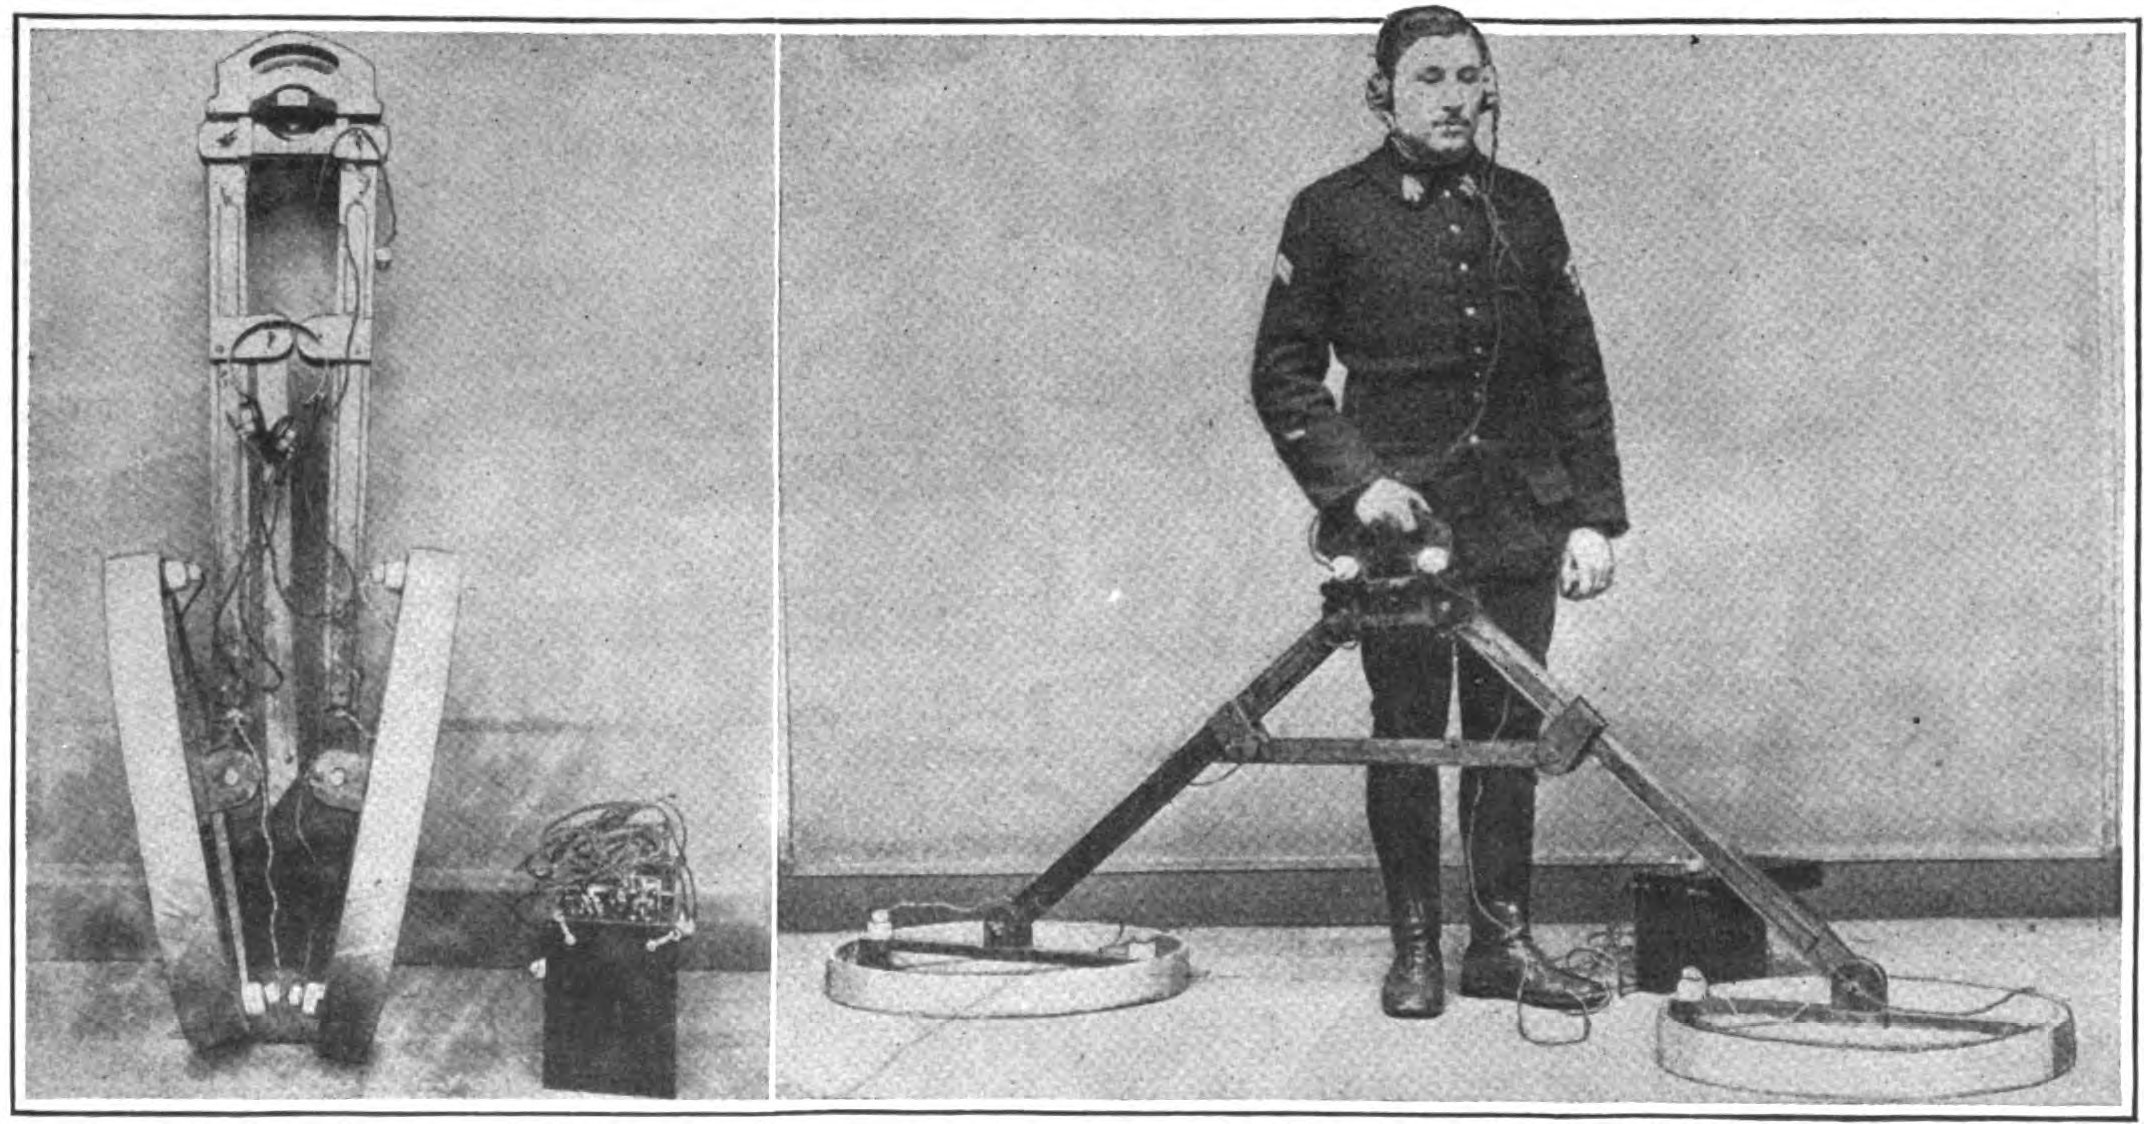
\includegraphics[width=21cm,keepaspectratio]{Pictures/Frontpage/Metal_detector_from_World_War_1.jpeg}};
\end{tikzpicture}

% Cover photo of us
\begin{figure}[b!]
    \captionsetup[subfigure]{font={sc,color=white}, labelformat=empty}
    \centering
    \vspace{1mm}
    \begin{subfigure}[1]{0.20\linewidth}
    
\includegraphics[width=\linewidth]{Pictures/Frontpage/Nikolaj.png}
    \captionsetup{justification=centering}
    \caption[]{{\small xxxnavnxxx}\\{insæt std}}
    \end{subfigure}
    \hspace{2em}
    \begin{subfigure}[1]{0.20\linewidth}
    
\includegraphics[width=\linewidth]{Pictures/Frontpage/Nikolaj.png}
    \captionsetup{justification=centering}
    \caption[]{{\small xxxnavnxxx}\\{insæt std}}
    \end{subfigure}
    \hspace{2em}
    \begin{subfigure}[1]{0.20\linewidth}
    
\includegraphics[width=\linewidth]{Pictures/Frontpage/Nikolaj.png}
    \captionsetup{justification=centering}
    \caption[]{{\small xxxnavnxxx}\\{insæt std}}
    \end{subfigure}
    \hspace{2em}
    \vspace{20mm}
\end{figure}
\end{titlepage}
\pagecolor{white}
\newgeometry{top=2.70cm, bottom=2.70cm, outer=2.5cm, inner=2.5cm}
\pagestyle{plain}
\clearpage
\renewcommand{\contentsname}{Indholdsfortegnelse} %This is the name of the content / Indholdsfortegnelse. Changing this will change it in the rapport.
\renewcommand{\figurename}{Figur}
\renewcommand\tablename{Tabel}
\tableofcontents
\clearpage

%%%%%%%%%%%%%%%%%%%%%%%%%%%%%%%%%%%%%%%%%%%%%%%%%%%%%%%
\pagenumbering{arabic}
\subfile{Chapters/01_Introduktion}
\clearpage
\subfile{Chapters/02_Analyse}
\clearpage
\subfile{Chapters/03_Design}
\clearpage
\subfile{Chapters/04_Implementering}
\clearpage
\subfile{Chapters/05_Test}
\clearpage
\subfile{Chapters/06_Konklusion}
\clearpage
%\subfile{Chapters/08_Colours}
%\clearpage
%\subfile{Chapters/09_eksempler}
%\clearpage
%\subfile{Chapters/10_Examples}
%%%%%%%%%%%%%%%%%%%%%%%%%%%%%%%%%%%%%%%%%%%%%%%%%%%%%%%

%\printbibliography[heading=bibintoc,title={Bibliography}]
\clearpage
\appendix
\chapter{Appendiks}
\section{Planlægning}

\subsection{Gantt-skema}
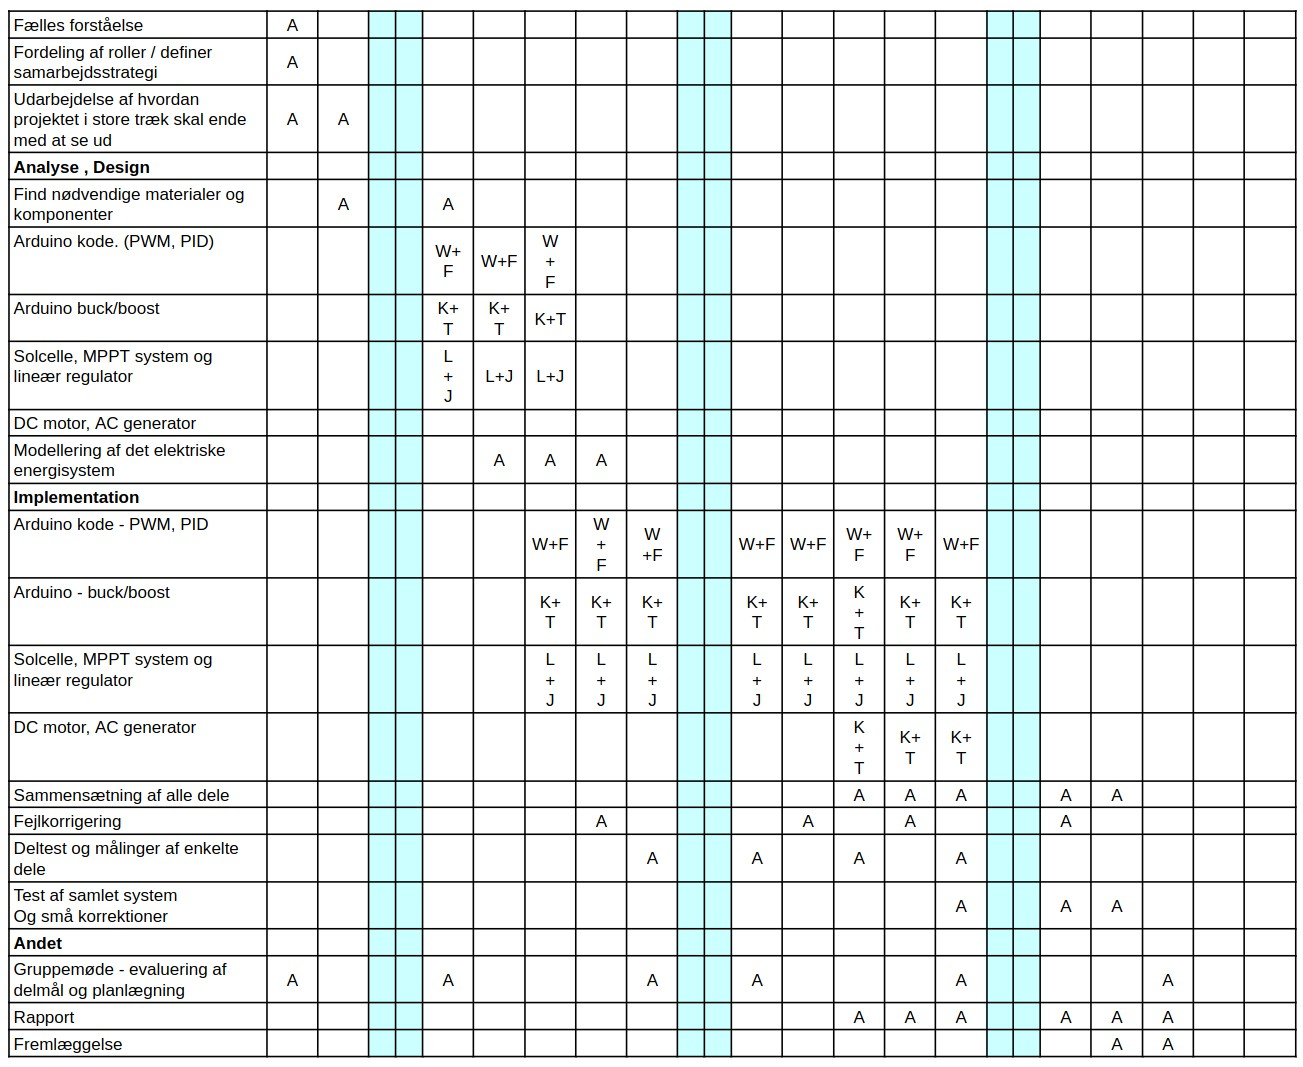
\includegraphics[width=\textwidth]{Dokumentation/Figures/Gantt Chart.jpg}
\label{fig: Gantt-Skema}
A: Alle \newline
W: Andreas Wendelboe\newline
F: Anders From\newline
K: Oliver Klinke\newline
T: Magnus Thorsteinsson\newline
L: Simon Lassen\newline
J: Jonas Frederiksen\newline
\clearpage
\section{Beregninger} \label{Chap:Beregninger}







\subsection{Transmitterspole/TX-spole}\vspace{5mm}
\underline{Anvendte konstanter}
\begin{align*}
    \mu_0  &= 1.25663706212 \cdot 10^{-6}\: \frac{H}{m}\\
    \rho_{Cu} &= 1.68 \cdot 10^{-8}\: \Omega \cdot m
\end{align*}

\underline{Valgte parametre}
\begin{align*}
    f_r &= 2.00 kHz\\
    r_{spole} &= 13.7cm\\
    A_{pk-pk} &= 8.00V
\end{align*}

\underline{Approksimation af sinusbølgens amplitude}
$$\boxed{a_n=2\cdot\frac{A}{n\cdot\pi}\cdot sin\left(\frac{n\cdot\pi}{2}\right)}$$
\begin{align*}
    a_1 &= 2\cdot\frac{8V}{\pi}\cdot sin\left(\frac{\pi}{2}\right) &= 5.09V\\
    a_{RMS} &= \frac{a_1}{\sqrt{2}} &= 3.60V
\end{align*}
Da kredsløbet udelukkende er resistivt ved resonans:
$$\;\quad R = \frac{a_{RMS}}{I} = \frac{3.60V}{250mA} \;\; \qquad \qquad \qquad = 14.4\Omega$$

\underline{Transmitterspolens antal vindinger}
$$\boxed{N_{TX}=\frac{R \cdot r_{wire}^2}{2 \cdot r_{coil} \cdot \rho}}$$
Ud fra de tilgængelige kobberledninger ($\rho = \rho_{Cu}$), vælges diameteren 0.355mm.
$$N_{TX} = \frac{14.4\Omega\cdot(\frac{0.355mm}{2})^2}{2 \cdot 13.7cm \cdot 1.68 \cdot 10^{-8}\:\Omega\cdot m} = 98.57 \approx 99$$
\underline{Valg af antal lag}\\
For at spolen og dermed spolehovedet ikke skal blive for højt vælges at spolen skal ligge i 5 lag ($n_{lag}=5$)\vspace{5mm}\\
\underline{Vidden af vindingerne (max)}
    $$\boxed{A_{vidde_{max}}= \left\lceil \frac{N_{TX}}{n_{lag}} \right\rceil \cdot d_{wire}}$$
\begin{align*}
    A_{vidde_{max}}&= \left\lceil \frac{99}{5} \right\rceil \cdot 0.355mm &\\
    &= \;\quad 20 \cdot 0.355mm &= 7.10mm
\end{align*}



\underline{Selvinduktans}
$$\boxed{L[\mu H] = \frac{0.394\cdot r_{spole}^2[cm]\cdot N_{TX}^2}{9\cdot r_{spole}[cm]+10\cdot A_{vidde}[cm]}}$$
$$ L_{TX} = \frac{0.394 \cdot 13.7^2 \cdot 99^2}{9 \cdot 13.7 + 10 \cdot 0.710}\mu H = 5.56mH$$
\underline{Kondensatorens kapacitans}
$$\boxed{f_r= \frac{1}{2\cdot\pi\cdot\sqrt{L \cdot C}} \Leftrightarrow C = \frac{1}{4\cdot\pi^2\cdot f_r^2\cdot L}}$$
$$C = \frac{1}{4\cdot \pi^2\cdot 2kHz\cdot 5.56mH} =1.14\mu F$$

\underline{B-felt}
$$\boxed{\lvert \overrightarrow{B} \rvert = \frac{\mu_0\cdot I\cdot N_{TX}}{2\cdot r_{spole}}}$$
$$\lvert \overrightarrow{B} \rvert = \frac{1.26\cdot10^{-6}\frac{H}{m}\cdot250mA\cdot 99}{2\cdot 13.7cm} = 113.5\mu T$$

\subsection{Modtagerspolen (RX)}
Kravspecifikationens pkt. 16 angiver min. 10mH selvinduktans for modtagerspolen.\\
Ved at angive en selvinduktans, der er dobbelt så stor som kravet, opnås en stor fejlmargin ved eventuelle afvigelser mellem teoretiske udregninger og virkelige forhold.
Med udgangspunkt i dette og med antagelsen af at modtagerspolen får samme vidde som transmitterspolen fås følgende:
\begin{align*}
    L_{RX} &= \frac{0.394\cdot 13.7^2\cdot N_{RX}^2}{9\cdot13.7+10\cdot0.71}\mu H & &=20000\mu H\\
           &= \frac{73.98\cdot N_{RX}^2}{130.43} \mu H                            & &=20000\mu H\\
    \lvert N_{RX} \rvert &= 187.8                                                 & &\approx 188
\end{align*}

\subsection{Modtagerspolen (RX)}
\begin{align*}
    L_{RX} &= \frac{0.394\cdot 13.7^2\cdot N_{RX}^2}{9\cdot13.7+10\cdot0.71}\mu H & &=20000\mu H\\
           &= \frac{73.98\cdot N_{RX}^2}{130.43} \mu H                            & &=20000\mu H\\
    \lvert N_{RX} \rvert &= 187.8                                                 & &\approx 188
\end{align*}
\clearpage
\section{Figurer}


\clearpage
\section{VHDL-kode}
%%\lstinputlisting[language=VHDL]{Files/VHDL/xxx.vhd}
\clearpage
\end{document}